% ******************************* Thesis Appendix C ********************************

\chapter{Statistical tools, models and plots}
\label{ap:stat_tools_models}

% **************************** Define Graphics Path **************************
\ifpdf
    \graphicspath{{Appendix3/Figs/Raster/}{Appendix3/Figs/PDF/}{Appendix3/Figs/}}
\else
    \graphicspath{{Appendix3/Figs/Vector/}{Appendix3/Figs/}}
\fi

%*****************************************************************************************
%*****************************************************************************************
\section{Statistical tools}
\label{sec:stat_tools}

This section introduces the common concepts, terms, notations, and methods that are used in multiple chapters. Those that appear in only a single chapter, for example interval analysis (see Section \ref{sec:uncertainty_rep_prop}), are introduced there.

%*****************************************************************************************
\subsection{Point estimates}
\label{subsec:point estiamtes}

Point estimates are single value ``guesses'' of population parameters from a sample. There are many methods to make point estimates, these can be compared by their properties such as bias, consistency, efficiency, and sufficiency \citep{Tsokos2009}. Here the method of moments, frequentist, and Bayesian methods are considered; all depends on the choice of the distribution function.

%..........................................................................................
\subsubsection*{Method of moments}
The method of moments (MM) is based on equating the sample and distribution moments: for a distribution with $n$ parameters the first $n$ moments are used. It is a widespread technique in civil engineering, which is applied in the Eurocode snow background document for fitting distributions and constructing characteristic ground snow maps \citep{Sanpaolesi1998}. It is a typically asymptotically unbiased though not in general efficient estimator \citep{Tsokos2009}. For stationary distributions moments are sufficient statistics; however, they are insufficient for non-stationary ones as they lack information about chronological order. This method is treated separately from statistical paradigms, since due to its simplicity it does not require commitment to any probability interpretation. 

Generalized method of moments (GMM) extends the notion of moments and can take into account more conditions than unknown parameters. Parameters are selected by minimizing the distance of sample and model moments while these conditions are weighted according to their relative importance to get an asymptotically efficient estimator \citep{Hall2005}. In this study the GMM parameter estimation is formulated as a just-identified problem, this means that the number of constraints is equal to the number of distribution parameters, and unbiased central moment constraints are adopted. Thus, only the asymptotic normality property is utilized to obtain the uncertainty intervals. The real strength of GMM lies in problems where the constraints are naturally set by the underlying theory and the distribution dependence can be avoided, for instance in some economics problems. GMM can be considered to be part of the frequentist approach; however, its separate treatment is explained by its connection to classical method of moments.

%..........................................................................................
\subsubsection*{Frequentist method}

The maximum likelihood (ML) method is used, which is typically an asymptotically efficient and consistent estimation technique that selects the model which is most likely generated the data \citep{Casella2001}. Inference of the unknown parameters, $\boldsymbol{\theta}$, is completed by maximizing the likelihood function, $L\left(\boldsymbol{\theta } \right)$:
\begin{equation}
\label{eq:max_like}
	L\left(\boldsymbol{\theta } \right) = \prod\limits_{i = 1}^n {p\left( {{x_i},{\boldsymbol{\theta }}} \right)}
\end{equation}
where $x_i$ denotes the observations, and $p(x)$ is the probability density function. In related methods and in numeric algorithms often the natural logarithm of the likelihood is applied, which is termed the log-likelihood function.

%..........................................................................................
\subsubsection*{Bayesian method}

The Bayesian approach is based on Bayes’ theorem, which compared with the frequentist approach additionally requires prior information on the unknown parameters:
\begin{equation}
\label{eq:bayes_rule}
\begin{split}
	p\left( {\left. {\boldsymbol{\theta }} \right|{\bf{x}}} \right) &= \frac{{prior \cdot likelihood}}{{evidence}} \\
	&= \frac{{p\left( {\boldsymbol{\theta }} \right) \cdot p\left( {\left. {\bf{x}} \right|{\boldsymbol{\theta }}} \right)}}{{p\left( {\bf{x}} \right)}} \\
	&= \frac{{p\left( {\boldsymbol{\theta }} \right) \cdot p\left( {\left. {\bf{x}} \right|{\boldsymbol{\theta }}} \right)}}{{\int\limits_{\boldsymbol{\Theta}}  {p\left( {\boldsymbol{\theta }} \right) \cdot p\left( {\left. {\bf{x}} \right|{\boldsymbol{\theta }}} \right) \cdot \mathrm{d}{\boldsymbol{\theta }}} }}.
\end{split}
%\begin{split}
%	f_{\boldsymbol{\Theta}|X}\left( {\left. {\boldsymbol{\theta }} \right|{\bf{x}}} \right) &= \frac{{prior \cdot likelihood}}{{evidence}} \\
%	&= \frac{{f_{\boldsymbol{\Theta}}\left( {\boldsymbol{\theta }} \right) \cdot f_{X|\boldsymbol{\Theta}}\left( {\left. {\bf{x}} \right|{\boldsymbol{\theta }}} \right)}}{{f_X\left( {\bf{x}} \right)}} \\
%	&=  \frac{{f_{\boldsymbol{\Theta}}\left( {\boldsymbol{\theta }} \right) \cdot f_{X|\boldsymbol{\Theta}}\left( {\left. {\bf{x}} \right|{\boldsymbol{\theta }}} \right)}}{{\int\limits_{\boldsymbol{\Theta}}  {{f_{\boldsymbol{\Theta}}\left( {\boldsymbol{\theta }} \right) \cdot f_{X|\boldsymbol{\Theta}}\left( {\left. {\bf{x}} \right|{\boldsymbol{\theta }}} \right)} \cdot \mathrm{d}{\boldsymbol{\theta }}} }}
%\end{split}
\end{equation}
where $\mathbf{x}$ contains observations (data) and $p\left( {\left. {\boldsymbol{\theta }} \right|{\bf{x}}} \right)$ is the posterior distribution of parameters.
The typically used Bayesian point estimate is the mean of the posterior distribution, it corresponds to minimum quadratic loss. It is a typically consistent, asymptotically efficient, and asymptotically unbiased estimator \citep{Gelman2003}. For practical cases with small sample size special care should be taken to the priors as those may have important effect on the inference.



%******************************************************************************************
\subsection{Interval estimates}
\label{sec:interval_estimates}


Point estimates are often accompanied by intervals to express parameter estimation uncertainty due to sampling variability.


%..........................................................................................
\subsubsection*{Method of moments}
We are not aware of any methods to quantify parameter estimation uncertainty using classical method of moments. However, for GMM the asymptotic normality of its estimator makes it possible to construct uncertainty intervals, these are approximate confidence intervals. A $p$-level confidence interval has the following meaning: if the population sampling is repeated infinitely many times and each time a specific interval is constructed around the point estimate, then $p$ proportion of these intervals would cover the true parameter of the generating distribution. Due to this repeated hypothetical sampling and focus on data variability this approach belongs to the frequentist paradigm. If confidence intervals for other than typical distribution parameters are needed then the model is formulated by the parameter in question, e.g. a specific fractile. The confidence intervals are constructed with a method similar to delta method -- detailed in the next section --, although here the weighting matrix plays the role of the observed Fisher information matrix (Eq.\ref{eq:delta_var}); for additional details see \citet{Chausse2010}. The weighting matrix is continuously updated in all GMM inferences in this study.


%..........................................................................................
\subsubsection*{Frequentist method}
The frequentist uncertainty interval is termed confidence interval, its definition is given in preceding section. The following three methods are used in this study to construct it:
\begin{itemize}
	\item Delta method: it is based on the observed Fisher information matrix and utilizes the asymptotic normality of the ML estimator \citep{Coles2001, Dorfman1938}.
	\item Profile likelihood method: it is based on maximizing the log-likelihood function considering all but one parameter to obtain a section/profile of the log-likelihood function, then utilizing some asymptotic property the confidence interval of the free parameter can be estimated. It is more accurate than the delta method but computationally more demanding \citep{Box1964, Coles2001}.
	\item Bootstrapping: it is the resampling of the empirical distribution function \citep{Efron1979, Efron1994}. The uncertainty intervals are obtained by taking the fractiles of the bootstrap sample. The resampled empirical distribution function is constructed with plotting position recommended by \citet{Cunnane1978}, and with linear interpolation among the points with no extrapolation from the data range. From the three methods this is the most accurate and computationally most expensive as well.
\end{itemize}

The presentation of these methods can be found in the referred literature, only the delta method is outlined here in more details since that is frequently used in later chapters. The delta method can be used to approximate the confidence interval of parameters, $\phi$, that are scalar function, $h(.)$, of inferred parameters, $\boldsymbol{\theta}$:
\begin{equation}
\label{eq:scalar_fun}
	\phi  = h\left( {{\boldsymbol{\theta }}} \right) \quad \mathbb{R}^n\mapsto\mathbb{R}.
\end{equation}
The maximum likelihood estimate of the derived parameter is obtained by substituting the maximum likelihood estimates of the inferred parameters into the scalar function:
\begin{equation}
\label{eq:delta_mode}
	\hat \phi  = h\left( {{\boldsymbol{\hat \theta }}} \right)
\end{equation}
where the maximum likelihood estimates are denoted by a hat, for example $\hat \phi$.
The variance of $\hat \phi$ can be approximated as:
\begin{equation}
\label{eq:delta_var}
	{\mathrm{Var}\left({\hat \phi} \right)} \approx {\nabla {h^{\mathrm{T}}\left({\boldsymbol{\hat \theta }} \right)} \cdot {\bf{I}}_{_{\mathrm{O}}}^{ - 1}\left({\boldsymbol{\hat \theta }} \right) \cdot \nabla {h\left({\boldsymbol{\hat \theta }} \right)}}
\end{equation}
where ${\mathbf{I}}_{_{\mathrm{O}}}$ is the observed Fisher information matrix, which is the approximate curvature matrix (Hesse matrix) of the negative log-likelihood function. The asymptotic sampling distribution of $\hat \phi$ is normal with mean and variance given in Eq.\ref{eq:delta_mode} and Eq.\ref{eq:delta_var} respectively:
\begin{equation}
	\hat \Phi \; \dot{\sim} \; {\cal N}\left({\hat \phi ,{\mathrm{Var}\left({\hat \phi} \right)}}  \right).
\end{equation}
The fractiles of this sampling distribution can be used as confidence interval endpoints.
%..........................................................................................
\subsubsection*{Bayesian method}
The Bayesian uncertainty interval is named $p$-level credible or posterior interval, $p$ denotes the probability that the inferred parameter is within the interval \citep{Gelman2003}. Two out of the infinitely many credible intervals are used in this study (Figure \ref{fig:credi_int_illu}):
\begin{itemize}
	\item the equal tailed interval (eqi) with the same probability to be below or exceed bounds and
	\item the highest density interval (hdi) with the largest minimum density value.
\end{itemize}

\begin{figure}[htbp!] 
	\centering    
	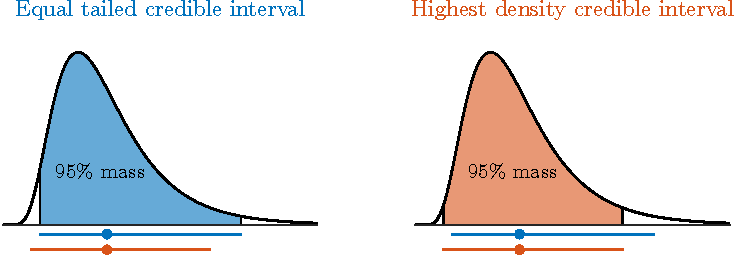
\includegraphics[]{credible_interval_illu_crop.pdf}
	\caption{Illustration of equal tailed and highest density credible intervals.}
	\label{fig:credi_int_illu}
\end{figure}



%******************************************************************************************
\subsection{Prediction}
Structural reliability is inherently predictive, for instance the design of a new structure is in large extent the prediction of future extreme actions and it should be based on a prediction appreciating the uncertainties stemming from scarcity of data, not just on a model that fits best to the observations.


%..........................................................................................
\subsubsection*{Frequentist method}
Many predictive likelihood based approaches are available in the literature \citep{Bjornstad1990}; however, there is no general agreement which one to use and they are rarely applied. Many of these approaches are similar to the Bayesian posterior predictive distribution (see next section) but they try to avoid the prior assumption. As Bayesian statistics is advocated in this study, predictive likelihood based approaches are not used in further chapters.

%..........................................................................................
\subsubsection*{Bayesian method}
An important advantage of the Bayesian approach is that it treats unknown parameters as random variables, hence the incorporation of parameter estimation uncertainty into the model is straightforward. This is done by averaging the conditional models, $p\left( {x|{\boldsymbol{\theta }}} \right)$, over the posterior distribution of the parameters, $p\left( {{\boldsymbol{\theta }}|data} \right)$ \citep{Gelman2003}:
\begin{equation}
\label{eq:postpred}
	p\left( x \right) = \int\limits_{\boldsymbol{\Theta}}  {p\left( {x|{\boldsymbol{\theta }}} \right) \cdot p\left( {{\boldsymbol{\theta }}|data} \right) \cdot \mathrm{d}} {\boldsymbol{\theta }}.
\end{equation}
The resulting function is referred to as posterior predictive, one of its interesting properties is that it automatically penalizes small sample size based predictions.


%****************************************************************************************** 
\subsection{Goodness-of-fit measures}
Once a model is fitted goodness-of-fit checks can be used to compare the data and model, and also to compare models. The former contains for instance P-P, Q-Q, return value-return period, and posterior predictive plots, these are detailed in Annex \ref{sec:prob_plots}, while the latter typically based on statistical tests or information theory measures. It is important that model-to-model comparisons do not guarantee good fit since it is a relative comparison and even the best model can perform poorly. Below only the information theory related measures are presented as those will be used in model averaging.


%..........................................................................................
\subsubsection*{Frequentist method}
The Akaike information criterion (AIC) is an asymptotic information criterion that is based on the premise that the model with smallest information loss (Kullback-Leibler divergence) should be preferred \citep{Akaike1973, Wit2012}. In the absence of the true model the information loss cannot be calculated in absolute terms; however, the models can be compared and their relative ``strength'' can be expressed by the difference in $AIC$s or by using Akaike weights (Eq.\ref{eq:Akaike_weight}). In this study the corrected form of Akaike information criterion (AICc) is applied that takes into account the effect of finite sample size \citep{Burnham2002}:
\begin{equation}
\label{eq:AIC}
	{AIC} = 2 \cdot k - 2 \cdot \ln \left( L \right)  \textrm{\quad and}
\end{equation}
\begin{equation}
\label{eq:AICc}
	{AICc} = {AIC} + \frac{{2k \cdot (k + 1)}}{{n - k - 1}}
\end{equation}
where $L$ is the likelihood; $k$ is the number of model parameters; and $n$ is the sample size. Akaike weight can be interpreted as the probability that a particular model is best in Kullback-Leibler divergence sense among the group of all considered models:
\begin{equation}
\label{eq:Akaike_weight}
	{w_i} = \frac{{\exp \left( {{{ - 1} \mathord{\left/
	 {\vphantom {{ - 1} {2 \cdot }}} \right.
	 \kern-\nulldelimiterspace} {2 \cdot }}AIC{c_i}} \right)}}{{\sum\nolimits_{j = 1}^K {\exp \left( {{{ - 1} \mathord{\left/
	 {\vphantom {{ - 1} {2 \cdot }}} \right.
	 \kern-\nulldelimiterspace} {2 \cdot }}AIC{c_j}} \right)} }}
\end{equation}
where $w_i$ is Akaike weight of the $i^\mathrm{th}$ model; and $K$ is the number of models under consideration.


%..........................................................................................
\subsubsection*{Bayesian method}
In the Bayesian paradigm goodness of a model is typically expressed as the probability of the model given the data. This probability for the $i^\mathrm{th}$ model ($M_i$) is conveniently denoted as $b_i$ and has a similar role as the Akaike weight \citep{Hoeting1999}:
\begin{equation}
\label{eq:bayes_weight}
	{b_i} = p\left( {{M_i}|data} \right) = \frac{{p\left( {\left. {data} \right|{M_i}} \right) \cdot p\left( {{M_i}} \right)}}{{\sum\nolimits_{j = 1}^K {p\left( {\left. {data} \right|{M_j}} \right) \cdot p\left( {{M_j}} \right)} }}
%	{b_i} = f_{X}\left( {{M_i}|data} \right) = \frac{{p\left( {\left. {data} \right|{M_i}} \right) \cdot p\left( {{M_i}} \right)}}{{\sum\nolimits_{j = 1}^K {p\left( {\left. {data} \right|{M_j}} \right) \cdot p\left( {{M_j}} \right)} }}
\end{equation}
where $p\left( {\left. {.} \right|{M_i}} \right)$ is the posterior predictive distribution for the $i^\mathrm{th}$ model. Since the integrals in Eq.\ref{eq:bayes_weight} can be difficult to compute often the Bayesian information criterion (BIC) is used for model selection:
\begin{equation}
	{BIC} = \ln \left( n \right) \cdot k - 2 \cdot \ln \left( L \right).
\end{equation}
It is an asymptotic information criterion that neglects prior distributions, the model with smallest $BIC$ should be preferred; for use of $BIC$ in model selection see \citet{Burnham2004}.
%\begin{equation}
%	b = \exp \left( -BIC/2 \right)
% \end{equation}
Both presented information criteria (AIC, BIC) penalize model complexity although with different weights. The penalization can be interpreted as Occam's razor to avoid over-fitting.



%******************************************************************************************
\subsection{Model averaging}
\label{subsec:model_averaging}
Since ``all models are wrong'' the goodness-of-fit measures typically do not clearly favor one model over the others. An approach to improve the fit and prediction is to average models based on their ``goodness''. Both frequentist and Bayesian paradigms offer averaging techniques, these of course yield to ``wrong'' models but by principle these are better than any of the individual models. Notice that the averaged model is conditioned on the pool of candidate models, thus its performance is dependent on them and does not guarantee good fit.

\mynote{GMM modela averaging, http://www.univie.ac.at/seam/inference/abstracts/luis_martins.pdf
Luis F. Martins GMM-based model averaging}

%..........................................................................................
\subsubsection*{Frequentist method}

In the frequentist paradigm the model averaged (FMA) point estimate is calculated as the weighted sum of the model parameters per different models \citep{Burnham2002}:
\begin{equation}
	\label{eq:FMA_point}
	\hat \theta  = \sum\nolimits_{i = 1}^K {{w_i} \cdot {{\hat \theta }_i}} 
\end{equation}
where the weight $w_i$ is the Akaike weight. Consensus on how to calculate the variance of the model-averaged parameters is missing. The following formula is used in this study \citep{Burnham2002}:
\begin{equation}
	\label{eq:FMA_var}
	\mathrm{Var} \left( {\hat \theta } \right) = \sum\nolimits_{i = 1}^K {{w_i} \cdot \left[ {\mathrm{Var}\left( {{{\hat \theta }_i}} \right) + {{\left( {{{\hat \theta }_i} - \hat \theta } \right)}^2}} \right]}.
\end{equation}
As the above equations (Eq.\ref{eq:FMA_point}-\ref{eq:FMA_var}) show the only requirement is that the averaged parameter is available in each model.


%..........................................................................................
\subsubsection*{Bayesian method}

In the Bayesian paradigm the model averaging (BMA) can be done with less ambiguity with any quantity of interest available in all models or directly on the level of distribution functions as well, weighting with model probabilities (Eq.\ref{eq:bayes_weight}): 
\begin{equation}
	\label{eq:BMA}
	p\left( x \right) = \sum\nolimits_{i = 1}^K {{b_i} \cdot {p\left( {x|{M_i}} \right)}}.
\end{equation}
Using the model averaged distribution $p\left( x \right)$ the desired parameters, e.g. mean value, can be readily calculated.


%..........................................................................................
\subsubsection*{Numerical considerations}

In general, the evaluation of the high-dimensional integrals needed in Eq.\ref{eq:bayes_rule} and thus in Eq.\ref{eq:BMA} is intractable. However, for small models up to 3-4 parameters -- as mostly considered here -- it can be readily calculated by numerical integration. It is worth mentioning that most probabilistic models in structural reliability are falling into this category, hence no significant computational limitation is expected. Moreover, as the tail of the distributions is of crucial importance, numerical integration is more efficient than standard Markov Chain Monte Carlo (MCMC) simulation techniques, which require a large number of simulations to adequately capture the tail.

Numerical comparisons using up to three-parameter distributions show that the numerical integration is computationally more efficient than the Metropolis-Hastings MCMC. The integration is implemented as a simple rectangular rule with parallelization, while the MCMC simulation is serial. The comparison is focused on estimating fractiles required in structural reliability, improvement is achieved by using affine invariant MCMC with ensemble sampler \citep{Goodman2010}, which takes advantage of parallel computing. Formulating of the distribution with the fractile in interest might yield to further improvement. Personal desktop computer is used for the comparison.

%*****************************************************************************************
%*****************************************************************************************
\section{Distribution functions}
\label{sec:distr_fun}

%****************************************************************
% Uniform distribution
\subsection*{Uniform distribution, $\boldsymbol{\mathcal{U}(a,b}$)}

\begin{equation}
	F(x)= \begin{cases} 0 & \text{for }x < a \\[8pt] \frac{x-a}{b-a} & \text{for }a \le x < b \\[8pt] 1 & \text{for }x \ge b \end{cases}
\end{equation}	
Where:

\begin{tabular}{ll}
	$a$ & left end of the interval, $[-\infty, \infty]$; \\
	$b$ & right end of the interval, $>a$.
\end{tabular}

%****************************************************************
% Normal distribution
\subsection*{Normal distribution, $\boldsymbol{\mathcal{N}(\mu,\sigma^2}$)}

\begin{equation}
	F(x,\mu ,\sigma ) = \frac{1}{2} \cdot \left( {1 + erf\left( {\frac{{x - \mu }}{{\sigma  \cdot \sqrt 2 }}} \right)} \right) = \Phi \left( {\frac{{x - \mu }}{\sigma }} \right)
\end{equation}	
Where:

\begin{tabular}{ll}
	$\mu$ & location parameter/mean, $[-\infty, \infty]$; \\
	$\sigma$ & scale parameter/standard deviation, $]0, \infty]$; \\
	$erf(.)$ & error function.
\end{tabular}

%****************************************************************
% Two-parameter lognormal distribution
\subsection*{Two-parameter lognormal distribution, $\boldsymbol{\mathrm{ln}\mathcal{N}(\mu,\sigma^2}$)}

%the last part is not correct !!!
\begin{equation}
	F(x,\mu ,\sigma ) = \frac{1}{2} \cdot \left( {1 + erf\left( {\frac{{\ln (x) - \mu }}{{\sigma  \cdot \sqrt 2 }}} \right)} \right) = \Phi \left( {\frac{{\ln (x) - \mu }}{\sigma }} \right)
\end{equation}	
Where:

\begin{tabular}{ll}
	$\mu$ & location parameter, $[-\infty, \infty]$; \\
	$\sigma$ & scale parameter, $]0, \infty]$.
\end{tabular}

%****************************************************************
% Three-parameter lognormal distribution 
\subsection*{Three-parameter lognormal distribution, $\boldsymbol{\mathrm{ln}\mathcal{N}(\mu,\sigma^2, \tau)}$}

\begin{multline}   
   F(x,\mu ,\sigma ,\tau ) = \int\limits_\tau ^x {\frac{1}{{\left( {x - \tau } \right) \cdot \sigma  \cdot \sqrt {2 \cdot \pi } }}} \exp \left[ {\left( { - \frac{1}{2} \cdot {{\left( {\frac{{\ln \left( {x - \tau } \right) - \mu }}{\sigma }} \right)}^2}} \right)} \right] \cdot \mathrm{d}x \\ = \Phi \left( {\frac{{\ln \left( {x - \tau } \right) - \mu }}{\sigma }} \right)
\end{multline}
Where:

\begin{tabular}{ll}
	$\mu$ & location parameter, $[-\infty, \infty]$; \\
	$\sigma$ & scale parameter, $]0, \infty]$; \\
	$\tau$ & shift parameter, $[-\infty, \infty]$.
\end{tabular}

%****************************************************************
% GEV distribution
\subsection*{Generalized extreme value distribution, GEV($\boldsymbol{\mu,\sigma,\xi}$)}

\begin{equation} \label{eq:gev_cdf}
	F(x,\mu ,\sigma ,\xi ) = \exp \left( { - {{\left( {1 + \xi  \cdot \left( {\frac{{x - \mu }}{\sigma }} \right)} \right)}^{{{ - 1} \mathord{\left/
						{\vphantom {{ - 1} \xi }} \right.
						\kern-\nulldelimiterspace} \xi }}}} \right)
\end{equation}	
Where:

\begin{tabular}{ll}
	$\mu$ & location parameter, $[-\infty, \infty]$; \\
	$\sigma$ & scale parameter, $]0, \infty]$; \\
	$\xi$ & shape parameter, $[-\infty, \infty]$.
\end{tabular}

%****************************************************************
% GEV distribution
\subsection*{Gumbel distribution, GUM($\boldsymbol{\mu,\sigma}$)}

Special case of GEV, can be obtained from Eq.\ref{eq:gev_cdf} by $\xi \to 0$.

%****************************************************************
%% Generalized pareto distribution
%\subsection*{Generalized Pareto distribution, GP($\boldsymbol{\mu,\sigma,\xi}$)}
%
%Cumulative distribution function of ${\left(X-u \right)}$, conditioned on $X$ is greater than a threshold, $u$:
%\begin{equation}
%	F(x,\mu ,\sigma ,\xi ) = 1 - {\left( {1 + \frac{{\xi  \cdot x}}{{\sigma  + \xi  \cdot (u - \mu )}}} \right)^{ - \frac{1}{\xi }}}
%\end{equation}
%Where:
%
%\begin{tabular}{ll}
%	$u$ & threshold parameter; \\
%	$\mu$ & location parameter, $[-\infty, \infty]$; \\
%	$\sigma$ & scale parameter, $]0, \infty]$; \\
%	$\xi$ & shape parameter, $[-\infty, \infty]$.
%\end{tabular}


%****************************************************************
% Nonstationary distributions


%****************************************************************
%% Maximum entropy distribution
%\subsection*{Maximum entropy distribution, ME(${\boldsymbol{\lambda }}$)}
%It is a non-parametric distribution that is based on the principle of maximum information entropy. By prescribing the equality of sample and distribution function's moments, the solution of the variational problem has the following form:
%\begin{equation}
%	f(x) = {e^{\sum\limits_{k = 0}^m {{\lambda _k} \cdot {x^k}} }}
%\end{equation}
%where:
%
%\begin{tabular}{ll}
%	$\lambda_k$ & distribution parameters; \\
%	$m$ & number of considered moments, $\geq 1$.
%\end{tabular}

% ALREADY GIVEN IN CHAPTER 8 IN A TABLE
%%****************************************************************
%% Copula function
%\section{Copula functions}
%Bivariate cumulative distribution functions of copulas are given below. If they exist they can be readily generalized to multidimensional cases, this is the case for Gauss and $t$ copulas.
%
%% Gauss copula
%\subsection*{Gauss}
%
%\begin{equation}
%	C(u_1, u_2) = {\Phi _2}\left( {{\Phi ^{ - 1}}({u_1}),{\Phi ^{ - 1}}({u_2});\theta } \right)
%\end{equation}
%Where:
%
%\begin{tabular}{ll}
%	$C(.)$	&	cumulative distribution function; \\
%	$u_1, u_2$ & independent variables, $[0,1]$; \\
%	$\theta$ & copula parameter, $[-1,1]$;  \\
%	$\Phi(.), \Phi_2(.)$ & univariate and bivariate normal cumulative distributions.
%\end{tabular}
%
%% t copula
%\subsection*{Student's \textit{t} (or simply \textit{t})}
%
%\begin{equation}
%	C(u_1, u_2) = {t_2}\left( {{t^{ - 1}}({u_1};\nu ),{t^{ - 1}}({u_2};\nu );\theta } \right)
%\end{equation}
%Where:
%
%\begin{tabular}{ll}
%	$\theta$ & copula parameter, $[-1,1]$; \\
%	$t(.), t_2(.)$ & univariate and bivariate $t$ cumulative distributions; \\
%	$\nu$ & degrees of freedom.
%\end{tabular}
%
%% Gumbel
%\subsection*{Gumbel}
%
%\begin{equation}
%	\begin{aligned}
%		C(u_1, u_2) &= \exp \left( { - {{\left( {{{\tilde u}_1}^\theta  + {{\tilde u}_2}^\theta } \right)}^{{1 \mathord{\left/
%	 	{\vphantom {1 \theta }} \right.
%	 	\kern-\nulldelimiterspace} \theta }}}} \right) \\
%	 	{\tilde u_i} &=  - \log \left( {{u_i}} \right)
%	 \end{aligned}
%\end{equation}
%Where:
%
%\begin{tabular}{ll}
%	$\theta$ & copula parameter, $[1,\infty]$.
%\end{tabular}
%
%% rotated Gumbel 180
%
%% rotated Clayton 180
%
%% F-H bounds
%

%****************************************************************
% Stochastic proceesses
%\section{Time-continuous stochastic processes}


%****************************************************************
\section{Probability plots}
\label{sec:prob_plots}

\subsection*{P-P plot}

A probability plot where theoretical and empirical cumulative distribution functions (probabilities) are plotted against each other. Closer the points to a 45$^\circ$ line closer the empirical distribution to the theoretical. Both distributions can be theoretical but only the former is used in this study.

\subsection*{Q-Q plot}

A probability plot where theoretical and empirical fractiles (quantiles) are plotted against each other. Closer the points to a 45$^\circ$ line closer the empirical distribution to the theoretical. Both distributions can be theoretical but only the former is used in this study.

\subsection*{Return period--return value plot}

Return period--return value plots are depicting cumulative distribution functions in specially transformed space where specific distribution types are forming a straight line. The plots are named after the related distribution type, for example Normal plot, Gumbel plot.
This  presentation  has  the  advantage  that:
\begin{itemize}
	\item it is easier  to  visually compare the models;
	\item deviation from the particular distribution type is clear;
	\item the crucial tail regions are enlarged by the logarithmic like scale of the horizontal axis.
\end{itemize}

The general form of the transformation:
\begin{equation*}
	F\left( {RV} \right) = P = 1 - \frac{1}{{RP}}\xrightarrow{transf.}RV = {a_1} \cdot \psi \left( {RP} \right) + {a_0}
\end{equation*}
Illustrating with Gumbel distribution:

\begin{equation*}
	\exp \left( { - \exp \left( { - \left( {\frac{{RV - \mu }}{\sigma }} \right)} \right)} \right) = 1 - \frac{1}{{RP}} \to RV =  - \sigma  \cdot {\ln}\left( { - {{\ln }}\left( {1 - \frac{1}{{RP}}} \right)} \right) + \mu
\end{equation*}

\begin{equation*}
\begin{split}
	\psi \left( {RP} \right) & =  - {\ln}\left( { - {{\ln }}\left( {1 - \frac{1}{{RP}}} \right)} \right) \\
	a_1 & = \sigma \\
	a_0 & = \mu.
\end{split}
\end{equation*}

Although $P=1-1/RP$ is a typical transformation between probabilities and return periods, it is not the only one. A theoretically more sound approach would be to assume that the extremes follow a Possion process, which implies exponentially distributed time between occurrences. Using this Poisson assumption the transformation:
\begin{equation*}
	P = \exp \left( { - \frac{1}{{RP}}} \right).
\end{equation*}

The comparison of these two transformations are presented in Figure~\ref{fig:RP_P_transform}. With the exception of the 1-10 year range, their difference in negligible; furthermore, the transformation only affect the visual appearance of plots.

\begin{figure}[htbp!] 
	\centering    
	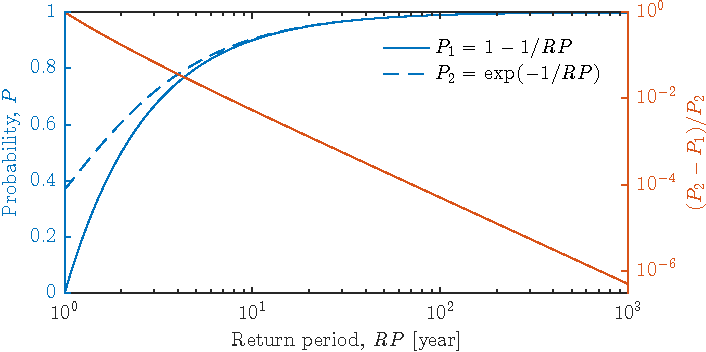
\includegraphics[]{RP_P_transform.pdf}
	\caption{Comparison of return period--probability transformations.}
	\label{fig:RP_P_transform}
\end{figure}